\documentclass[twocolumn]{aastex631}
\usepackage{graphicx}
\usepackage{float}

\begin{document}

\title{Angular Momentum Alignment Between Stellar Remnants and Dark Matter Halos in Galaxy Mergers}
\author{Ben A Phan}
\date{May 08, 2025}

\begin{abstract}
    Angular momentum alignment between stellar structures and their surrounding dark matter halos is a key factor in shaping galactic dynamics and morphology. This alignment is often disturbed during major mergers, leading to long-term kinematic consequences. In this project, we use a VLowRes simulation of the Local Group to track the angular momentum vectors of the stellar and halo components during the Milky Way–Andromeda merger. We examine how their orientations evolve, quantify misalignment, and assess whether realignment occurs post-merger. We find that the components begin significantly misaligned, become more disturbed during the merger phase, and show partial but incomplete realignment in the remnant structure. These results highlight the dynamical fragility of angular momentum structure during mergers and suggest that full recovery is unlikely within the simulated timescale. This has significant implications for understanding how mergers affect the structural and rotational properties of galaxies.
\end{abstract}




\keywords{Galaxy --- Galaxy Evolution --- Stellar Disk --- Dark Matter Halo --- Major Merger --- Angular Momentum --- Hernquist Profile --- Dynamical Friction --- Tidal stripping/sharing --- N-body Simulation}

\section{Introduction}

\subsection{Angular Momentum Alignment in Galaxy Mergers}

Angular momentum alignment between stellar structures and their surrounding dark matter halos plays a critical role in galaxy morphology and dynamics. During galaxy mergers, angular momentum is redistributed through processes like \textbf{tidal stripping/sharing}—the removal or exchange of weakly bound material—and \textbf{dynamical friction}, where massive bodies lose momentum via gravitational interactions. These mechanisms often cause misalignment between baryonic and dark matter components.

This study focuses on the Milky Way–Andromeda (MW–M31) system to track how angular momentum vectors of their dark matter halos and stellar disks evolve before, during, and after a \textbf{major merger}, defined as an interaction between galaxies with baryonic mass ratios between 1:1 and 1:4; \citep{Lotz2011}. The goal is to determine whether halo–disk alignment is preserved or disrupted by such events.

\subsection{Relevance to Galaxy Evolution}

Understanding halo–disk angular momentum alignment informs our models of galaxy evolution, structure, and rotational support. A \textbf{galaxy} is ``a galaxy is a gravitationally bound collection of stars whose properties cannot be explained by a combination of baryons and Newton’s laws of gravity." \citep{Willman2012}. The \textbf{stellar disk} forms the rotationally supported, flattened component of a galaxy, composed primarily of stars and gas, and is responsible for much of its visible structure and ordered rotation, while the \textbf{dark matter halo} is ``a virialized, extended structure decoupled from the universe’s expansion that gravitationally attracts baryons and enables galaxy formation" (private communication, G. Besla, 2025).

\textbf{Galaxy evolution} involves processes like mergers, gas accretion, and tidal interactions that reshape morphology and kinematics. A central tool in this analysis is the \textbf{angular momentum} vector:
\[
\vec{L} = \sum_i m_i (\vec{r}_i - \vec{r}_{\text{COM}}) \times (\vec{v}_i - \vec{v}_{\text{COM}})
\]
where $m_i$ is particle mass and $\vec{r}_i$, $\vec{v}_i$ are position and velocity relative to the component’s center of mass.

To characterize dark matter structure, we apply the \textbf{Hernquist profile}:
\[
\rho(r) = \frac{M}{2\pi} \frac{a}{r(r+a)^3}
\]
where $M$ is total mass and $a$ is the scale radius. This profile ensures finite mass and helps define a stable core for angular momentum measurement \citep{Hernquist1990}.

\subsection{Background and Open Questions}

Recent work shows that angular momentum alignment is sensitive to a galaxy’s merger history. \citet{Somerville2008} emphasized the importance of realistic dark matter halo models in reproducing observed galaxy growth. \citet{RodriguezGomez2017} showed that major mergers can significantly alter galaxy spin and morphology, while \citet{Lagos2018} demonstrated that mergers play a key role in shaping the stellar angular momentum content of galaxies.


\begin{figure}[H]
    \centering
    \includegraphics[width=0.45\textwidth]{figure5.png}
    \caption{Evolution of average disk sizes normalized to present-day sizes as a function of redshift, with circles representing more detailed halo profiles. The gradual evolution agrees with observations and reflects the predictive power of realistic halo modeling. Adapted from \citet{Somerville2008}.}
    \label{fig:somerville_fig5}
\end{figure}

Despite this progress, key questions remain: How does angular momentum alignment evolve through mergers? What determines whether halo–disk alignment is maintained or lost? Can remnants realign after coalescence? This project addresses these questions using a cosmological simulation of a major merger event.


\section{This Project}

\subsection{Project Overview}

This project investigates the angular momentum alignment between the dark matter halo and stellar disk components of the Milky Way (MW) and Andromeda (M31) galaxies throughout their merger. Using a VLowRes simulation of the Local Group, we track the angular momentum vectors of both components from $t = 0$ to $\sim12$ Gyr across 17 snapshots (0.5 Gyr intervals). We define the halo as particles within $r < 63$ kpc and the disk as those within $r < 15$ kpc to avoid contamination from loosely bound material. After $t \sim 6.5$ Gyr, when MW and M31 fully coalesce, we compute the angular momentum of the remnant. This allows us to evaluate whether the halo–disk alignment recovers or remains disrupted.

\subsection{Research Question}

This project asks: How does angular momentum alignment evolve through a major merger? Specifically, we examine whether the halo and disk components maintain, lose, or recover alignment during and after the MW–M31 merger. This question is central to galaxy evolution because angular momentum coherence affects disk regrowth, remnant morphology, and kinematic stability. By tracking this alignment over time, we assess how mergers reshape galactic structure.

\subsection{Method Overview}

We analyze simulation data using the following approach:

\begin{enumerate}
    \item \textbf{Component Selection}: Use particle type and radial cutoffs to isolate halo and disk components.
    \item \textbf{Center of Mass Frame}: Compute center-of-mass (COM) positions and velocities at each snapshot.
    \item \textbf{Angular Momentum Calculation}: Measure angular momentum vectors in the COM frame.
    \item \textbf{Alignment Tracking}: Calculate the angle between current and initial angular momentum vectors, and between halo and disk vectors over time.
    \item \textbf{Post-Merger Remnant}: Combine MW and M31 particles after $t \sim 6$ Gyr to analyze the remnant’s angular momentum.
\end{enumerate}

\section{Methodology}

\subsection{Simulation Overview}

We use the VLowRes Local Group simulation provided by \cite{vanderMarel2012}, which models the gravitational evolution of the Milky Way (MW) and Andromeda (M31) galaxies through their eventual merger.


This simulation is an example of an \textbf{N-body simulation}, where the gravitational evolution of a collisionless system is modeled using a finite number of tracer particles \citep{Springel2005}. In this case, the particles represent the stellar and dark matter components of each galaxy.

Each galaxy is initially modeled as:
\begin{itemize}
    \item Type 1: Dark matter halo particles, following a Hernquist profile \citep{Hernquist1990}, with scale radius $a \approx 63$ kpc, measured at snapshot 0 and held fixed throughout the simulation. This density profile provides total mass and replicates the inner structure of observed halos by modeling the radial mass distribution in three-dimensional space using spherical coordinates.
.
    \item Type 2: Stellar disk particles, selected within a radial cutoff of $r < 15$ kpc to focus on the rotationally supported baryonic structure. This simulation also includes a similar data set to the dark matter halo particles.
\end{itemize}

The simulation provides outputs at 800 Myr intervals, including particle data snapshots and orbital tracking files. The initial halo masses are $M_{\text{MW}} \sim 10^{12} M_\odot$ and $M_{\text{M31}} \sim 1.6 \times 10^{12} M_\odot$, providing sufficient resolution to track angular momentum evolution throughout the merger.


\subsection{Method Summary and Diagnostics}

This project follows a multi-step method, including particle selection, angular momentum calculations, and diagnostic plotting.

\textbf{1. Load and Classify Particles}: At each snapshot, we load positions and velocities using `ReadFile.py`. We classify type 1 (halo) and type 2 (disk) particles and apply radial cutoffs of $r < 63$ kpc for halos and $r < 15$ kpc for disks.

\textbf{2. Compute Angular Momentum}: For each component, we compute the center of mass using `CenterOfMass.py`, and then calculate angular momentum vectors:
\[
\vec{L} = \sum_i m_i (\vec{r}_i - \vec{r}_{\text{COM}}) \times (\vec{v}_i - \vec{v}_{\text{COM}})
\]

\textbf{3. Track Alignment Over Time}: To evaluate orientation changes, we compare $\vec{L}_t$ to the initial vector $\vec{L}_0$:
\[
\theta_t = \cos^{-1}\left( \frac{ \vec{L}_t \cdot \vec{L}_0 }{ |\vec{L}_t||\vec{L}_0| } \right)
\]
and calculate halo–disk misalignment:
\[
\phi_t = \cos^{-1}\left( \frac{ \vec{L}_\text{halo} \cdot \vec{L}_\text{disk} }{ |\vec{L}_\text{halo}||\vec{L}_\text{disk}| } \right)
\]

\textbf{4. Analyze Merger Remnant}: After $t \sim 6$ Gyr, MW and M31 are merged. We recompute COM and angular momentum for the remnant system.

\textbf{Figure Description}: We present one diagnostic plot showing the misalignment angle $\theta$ over time for each galaxy, without applying corrections. This draft figure helps identify sources of error in measurement frames and outer-region bias.

\begin{figure}[H]
    \centering
    \includegraphics[width=0.45\textwidth]{Angular_Momentum_MW_M31_Merger_No_Alignment_Boundary.png}
    \caption{Draft figure: Instantaneous angle $\theta$ between halo and stellar angular momentum vectors for MW, M31, and the merger remnant over time, without applying edge-on reorientation or inner boundary cutoffs. The absence of corrections leads to large discrepancies between galaxy components, emphasizing the importance of proper measuring frame alignment and particle selection.}
    \label{fig:draft_halo_disk_angle}
\end{figure}

\textbf{Future Work}: A corrected plot will incorporate edge-on disk reorientation and proper boundary limits. This will allow meaningful interpretation of angular momentum coupling throughout the merger process.


\subsection{Hypothesis}

We hypothesize that:
\begin{itemize}
    \item MW and M31 start with moderate halo–disk alignment.
    \item Dynamical friction and tidal interactions during the merger disrupt this alignment.
    \item After coalescence, partial realignment occurs, but full restoration of coherence is unlikely.
    \item Stellar components are more affected by the merger compared to dark matter components, and thus they contribute more significantly to shifts in angular momentum alignment during and after the merger.
\end{itemize}

\section{Results}

We present two figures that illustrate the evolution of angular momentum alignment between the stellar and dark matter halo components of the Milky Way (MW), Andromeda (M31), and the resulting merger remnant. The first shows how the halo–disk angular momentum angle evolves during the merger process, while the second tracks the orientation of each component (halo and disk) relative to its initial angular momentum direction. Together, these figures investigate how the merger event alters angular momentum alignment and identify which components contribute most to the misalignment during and after the interaction.

\begin{figure}[h!]
    \centering
    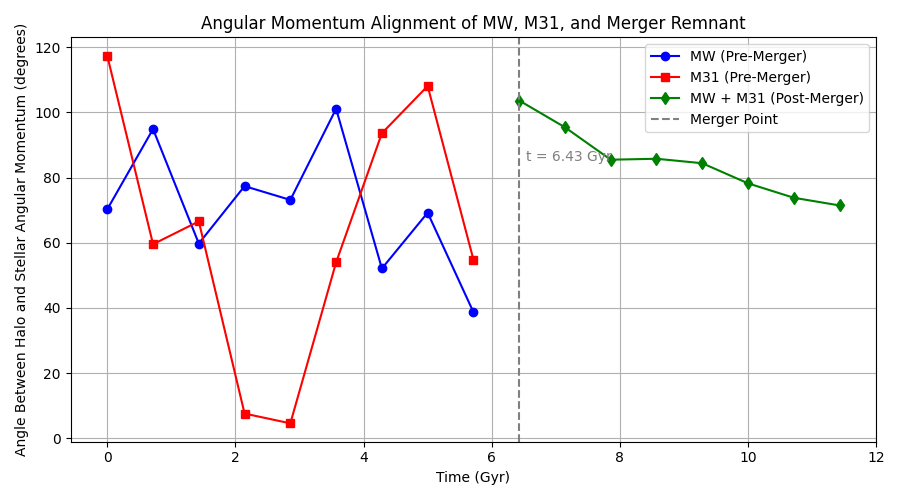
\includegraphics[width=0.9\linewidth]{Angular_Momentum_MW_M31_Merger.png}
    \caption{Angular momentum misalignment angle between halo and disk components for MW (blue), M31 (red), and the merger remnant (green) as a function of time. Unlike the draft result in Figure~\ref{fig:draft_halo_disk_angle}, this figure applies edge-on disk reorientation and radial cutoffs (63 kpc for halo, 15 kpc for disk), correcting for outer-region bias and inconsistent measurement frames. The merger occurs near 6.43 Gyr, with significant disruption between 2--4 Gyr. After the merger, the remnant shows improved alignment stability.}
    \label{fig:halo_disk_alignment}
\end{figure}

\subsection{Halo-Disk Alignment Over Time}

Figure~\ref{fig:halo_disk_alignment} shows the angle between the halo and stellar angular momentum vectors for MW, M31, and the merger remnant as a function of time. Initially, MW and M31 show significant misalignment (around 70$^\circ$ and 120$^\circ$, respectively). A sharp disruption occurs during 2--4 Gyr, especially for M31. We define the merger to occur when the separation between the two galaxies falls below 30 kpc, which happens at approximately 6.43 Gyr. After the merger, the remnant shows gradual stabilization, with halo–disk alignment fluctuations decreasing over time.




\subsection{Component Alignment Relative to Initial Directions}
\begin{figure}[h!]
    \centering
    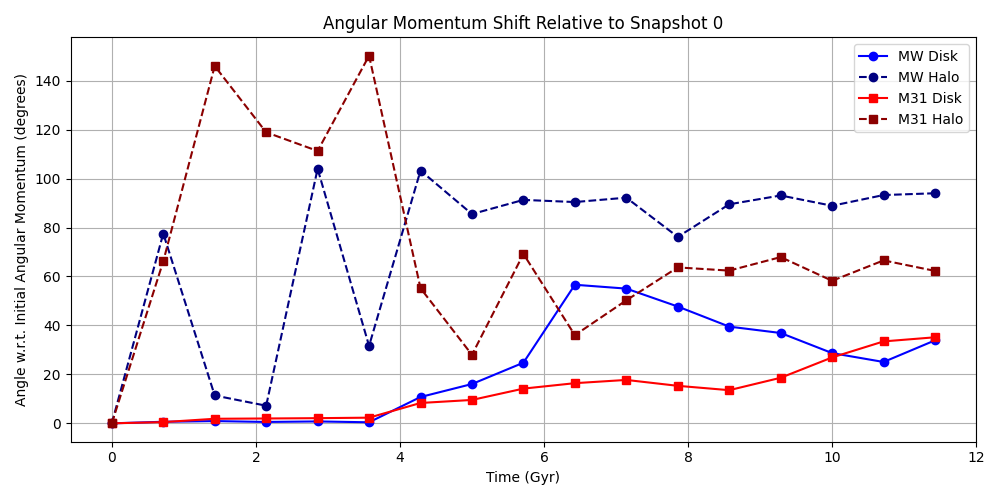
\includegraphics[width=0.9\linewidth]{Angular_Momentum_Relative_To_Initial.png}
    \caption{Evolution of the angular momentum vectors of MW and M31 halos and disks relative to their initial directions. During the merger phase (2--4 Gyr), halos experience greater reorientation than disks. After coalescence ($t \sim 6.43$ Gyr), components partially realign but do not fully recover their original orientations.}
    \label{fig:relative_alignment}
\end{figure}

Figure~\ref{fig:relative_alignment} tracks the evolution of the halo and disk angular momentum vectors for MW and M31 relative to their initial directions at $t = 0$ Gyr. Both halos and disks experience significant reorientation during the merger phase (2--4 Gyr), consistent with the period during which Figure~\ref{fig:halo_disk_alignment} shows greatest alignment disturbance. Notably, the halos reveal larger fluctuations in alignment compared to the disks, suggesting that the dark matter components contribute more to the misalignment of both galaxies in Figure~\ref{fig:halo_disk_alignment} and are more sensitive to gravitational perturbations. After the merger, the remnant components show partial realignment toward their original angular momentum directions, but full recovery is not achieved during the 12 Gyr timeframe of this simulation.


\section{Discussion}

Our results confirm that major mergers cause substantial misalignment between halo and stellar angular momentum components. The large initial misalignment observed in MW and M31 ($\sim$70$^\circ$ and $\sim$120$^\circ$, respectively) suggests their halos and disks were already kinematically decoupled prior to merging, possibly due to differing formation histories or prior interactions.

These findings align with previous work \citep{Zavala2008}, emphasizing that angular momentum structures are fragile and easily disturbed. The merger phase (2–4 Gyr) produces sharp disruptions, but the remnant shows some stabilization post-merger. Still, full angular momentum realignment is not achieved.

Interestingly, our analysis shows that dark matter halos are more disrupted than stellar disks, contrary to the hypothesis that stellar components would be more sensitive. This reflects the more extended, loosely bound nature of halos, making them more responsive to tidal torques and dynamical friction. Our result is consistent with \cite{Zavala2008}, who showed that dark matter halos lose a significant fraction of their angular momentum during mergers, while baryonic components (especially in disc-dominated galaxies) tend to preserve theirs.

Several uncertainties may affect our results. First, the Hernquist scale radius was fixed from snapshot 0 and applied throughout the simulation, even after the merger. Since the density structure evolves during the interaction, this static cutoff could introduce errors in halo particle selection, especially post-merger. We also define merger completion as the moment when the Milky Way and Andromeda reach a physical separation of 30 kpc. This threshold provides a convenient and observationally motivated marker for merger timing, but its physical accuracy remains somewhat debatable and may vary between different systems. For example, \citet{Lotz2011} defines close galaxy pairs observationally using projected separations in the range of 10–30 $h^{-1}$ kpc (approximately 14–43 kpc for $h = 0.7$), which aligns with the 30 kpc cutoff adopted in this work. Therefore, while this choice is not based on a physically derived threshold, it follows standard practice in observational studies and provides a reasonable estimate for when coalescence begins.
 The absence of M33’s gravitational influence and the lack of baryonic physics (e.g., gas, feedback) in the simulation also limit the realism of our conclusions. Finally, our radial cutoffs (63 kpc for halo, 15 kpc for disk) are approximations and may exclude particles contributing meaningfully to angular momentum.

Despite these limitations, our central conclusion is clear: major mergers significantly disrupt angular momentum alignment, and full recovery is not guaranteed even several Gyr after coalescence.

\section{Conclusions}
Major mergers significantly impact the angular momentum alignment between dark matter halos and stellar disks, a key driver of galaxy structure. This project explored how such alignment evolves through the Milky Way–Andromeda merger using VLowRes simulation data. 

Our analysis reveals that halos and stellar components begin moderately aligned, become highly misaligned during the 2–4 Gyr merger window, and only partially realign afterward. This supports our hypothesis that angular momentum coherence is disrupted by dynamical friction and tidal forces, though halos were unexpectedly more affected than disks.

Future work could explore this further using higher-resolution simulations with baryonic physics and incorporating additional galaxies like M33. Adding gas dynamics and feedback processes would improve the realism of angular momentum modeling in merger remnants.

\section*{Acknowledgements}
I thank Professor Gurtina Besla and Himansh Rathore for their guidance throughout this project. This work made use of the following open-source Python libraries: \texttt{Astropy} \citep{astropy2013,astropy2018}, \texttt{matplotlib} \citep{hunter2007}, \texttt{numpy} \citep{vanderwalt2011}, \texttt{scipy} \citep{jones2001}, and \texttt{IPython} \citep{perez2007}. Portions of this report were drafted and revised with assistance from ChatGPT (OpenAI, 2024), and I confirm all content was reviewed and understood.

We respectfully acknowledge the University of Arizona is on the land and territories of Indigenous peoples, including the O’odham and the Yaqui.

\bibliography{cite.bib}
\bibliographystyle{aasjournal}

\end{document}